\documentclass{article}
\usepackage[utf8]{inputenc}
\usepackage{amsmath}
\usepackage{enumitem}
\usepackage{graphicx}
\usepackage{framed}
\usepackage{listings}
\usepackage{pdfpages}
\usepackage{caption}
\usepackage{subcaption}
\usepackage[utf8]{inputenc}
\usepackage{minted}
\usepackage{placeins}
\usepackage[utf8]{inputenc}


\title{Ch 9 Group Part 2}
\author{Tate Meehan, Arash Modaresi Rad, William Rudisill}
\date{March 2019}

\begin{document}

\maketitle

\section{Equation}
The Van Genuchten equation is used to model volumetric soil water content as a function of pressure head: 
\begin{align}
\theta = \theta_r + \frac{\theta_s - \theta_r}{\big(1 + \alpha h^n\big)^m}
\end{align}

\section{Part 1}
\subsection{a.}

\begin{table}[!h]
\caption{The optimal parameters of the van Genuchten equation for soil 1420.}
\begin{tabular}{|c|c|c|c|c|}
\hline
$\mathbf{m_1} = \alpha$      & $\mathbf{m_2} = n$    & $\mathbf{m_3} = m$     & $\mathbf{m_4} = \theta_s$   & $\mathbf{m_5} = \theta_r$    \\ \hline
$0.0038 \pm 0.0004$ & $1.1621\pm0.0439$ & $0.3320 \pm 0.040$ & $0.5331\pm0.001$ & $0.1370\pm0.0110$ \\ \hline
\end{tabular}
\label{tab:2a}
\end{table}
\vspace{-20pt}
\subsection{b.}
\begin{figure}[!h]
    \centering
    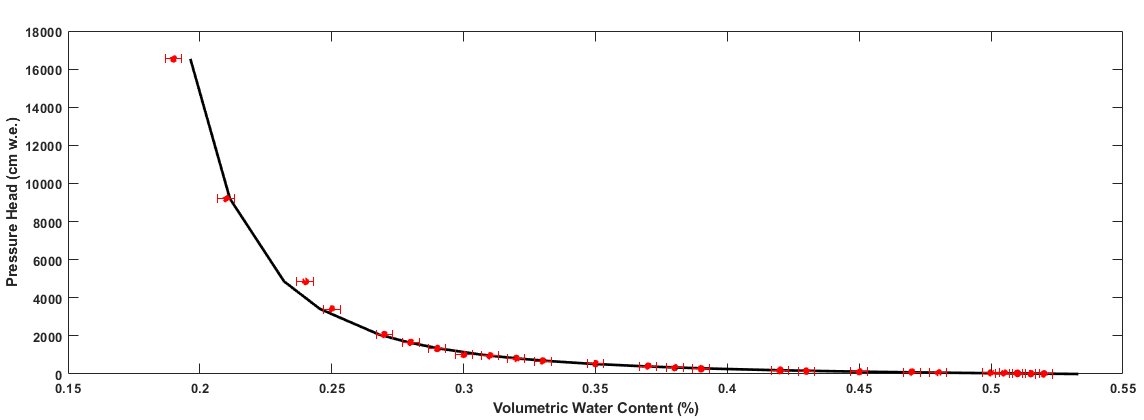
\includegraphics[width=\textwidth]{2a.png}
    \caption{The water retention plot of soil code 1420 obtained from the UNSODA database.The black line is the fitted model, the red points indicate observations and data standard deviation are estimated from posterior fit.}
    \label{fig:2b}
\end{figure}

\subsection{c.}
The observed p-value is 0.461 with a $\chi^2$ statistic of 23.00 and 23 degrees of freedom. This implies that there is a 46.1 percent chance that one might obtain a solution with a worse data fit. There are some caveats however. We do not have the population data with which to estimate the data standard deviation. We therefore estimate the data standard deviation ($\sigma^2$) from the model residual fit (equation 2.69 from the book). The consequence is that the model parameter estimates are not as tightly constrained (the model parameter estimates follow a t-distribution as opposed to a normal distribution).  

\subsection{d.}
The estimate of the covariance of the model parameters are given by:

\begin{equation}
Cov(m^*) = (J(m^*)^TJ(m^*))^{-1}
\end{equation}
We find the following covariance structure for our model parameters: 
\begin{figure}[ht!]
    \centering
    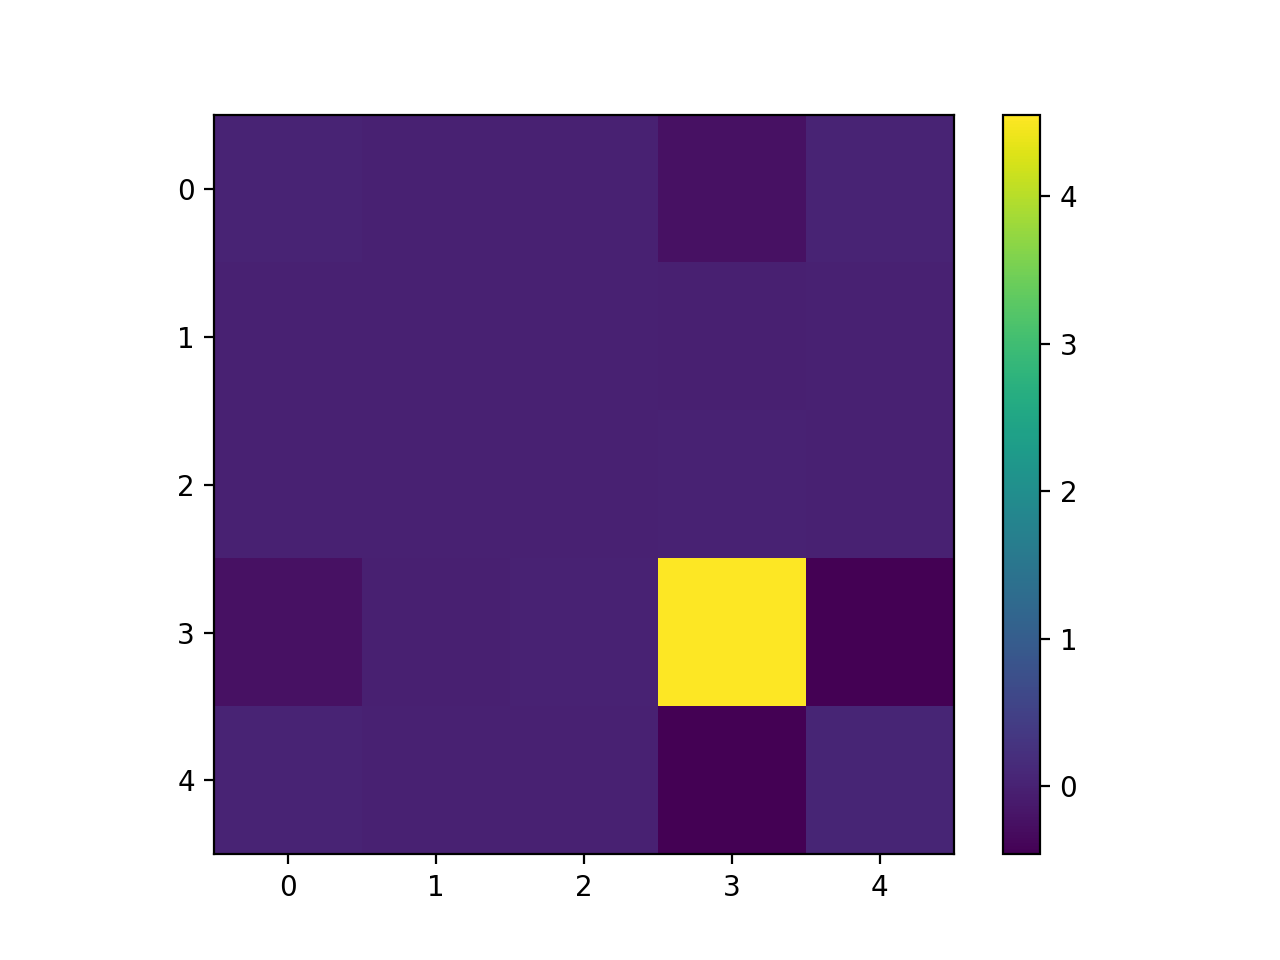
\includegraphics[width=\textwidth]{2d_covar_matrix.png}
    \caption{Covariance structure for the model parameters}
    \label{covarmat}
\end{figure}
Interestingly, there is a large covariance structure (and thus confidence interval) for the 3rd model parameter (Figure \ref{covarmat}). This corresponds with the model parameter "m" from equation 1. This implies that the there is a large degree of uncertainty in the $m^*$ estimate for this parameter. 

\newpage

\subsection{e.}
Figure \ref{contours} shows contour plots of the chi-square surface for various ranges of model parameter pairs. We can see that that the contours do not form ellipses, indicating that we are dealing with a non-linear system. 


\begin{figure}[!hb]
    \centering
    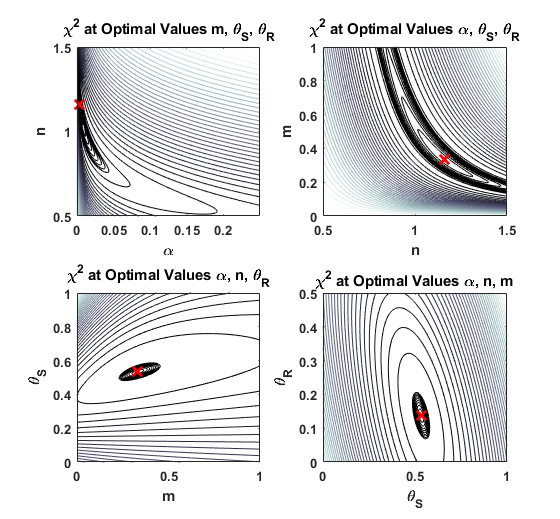
\includegraphics[width = 0.85\textwidth]{2e.png}
    \caption{The $\chi^2$ objective function is plotted for two parameters while fixing the remaining three parameters at the optimal values presented in Table \ref{tab:2a}. The red X indicates the location of the optimal parameters. The quality of the ellipsoid for the upper two plots indicates a moderate degree of nonlinearity at the parameter values. The lower plots display a regular ellipse shape at the estimated parameters indicating the linear approximation near the solution is good. }
    \label{contours}
\end{figure}


% \begin{table}[ht!]
%     \centering
%     \begin{tabular}{c|c}
%          &  \\
%          & 
%     \end{tabular}
%     \caption{Caption}
%     \label{tab:my_label}
% \end{table}

\subsection{f.}
Choosing initial model parameters can be challenge due to the presence of local minima. Selecting reasonable starting guesses for model parameters is one way of imposing a priory knowledge into the parameter estimate from inversion. Figure \ref{fig:2f} shows model parameter estimates from a range of starting vectors (n=50). We were able to find parameter estimates that are reasonable given our knowledge of the physical system. 


\begin{figure}
    \centering
    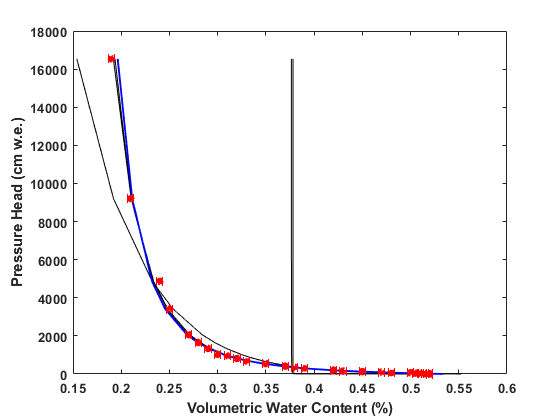
\includegraphics[width=0.85\textwidth]{2f.png}
    \caption{Of 50 randomly chosen starting parameters from a uniform distribution between 0 and 1 approximately 15 - 20 of the solutions are accepted under the criteria that the solution is in the real plane and that the solution met convergence. The 0-1 domain is a realistic scenario of the neighborhood for the optimal parameters. Three modes for solutions appear in black. Our chosen curve is blue, the curves that agree well with the blue curve have parameters that also agree well, within the bounds of the 95\% confidence interval provided in Table \ref{tab:2a}. }
    \label{fig:2f}
\end{figure}


\newpage
Matlab Codes
\begin{minted}{matlab}
%% Group Assignment Chapter 9
clear; close all; clc;
%% 
global theta;
global h;
global sigma;
[h] = xlsread('soil.xlsx','sheet1','B2:B29');
theta = xlsread('soil.xlsx','sheet1','C2:C29');
sigma = std(theta);
% sigma = 1;
h(1) = 0.00001;
% p0 = ([1,1,1,.6,.1]');
% Parameters from table
% m = 1/(exp(.182)-1)
% p0 = [exp(-2.076),exp(.182),1,.482,.090]';
% Guess with Weighting
p0 = ([.01,1,1,1,1]')./2;

tol = eps.^(.125);
maxiter = 1000;

[pstar, iter] = lm('fun', 'jac', p0, 0.0001, maxiter);

goodWill =  vanGenuchten(pstar);

% Posterior Standard Deviation Estimate
dof = length(h) - 5;
s = norm(goodWill - theta)./sqrt(dof);

figure();plot((goodWill),(h),'k','linewidth',2);
hold on; errorbar((theta),(h),(ones(length(theta),1).*s./2),'horizontal','or','markerfacecolor','r','markersize',5);
xlabel('Volumetric Water Content (%)')
ylabel('Pressure Head (cm w.e.)')
set(gca,'fontweight','bold')
% figure();plot(log(goodWill),log(h),'k','linewidth',2);
% hold on; errorbar(log(theta),log(h),(ones(length(theta),1).*s./2),'horizontal','or','markerfacecolor','r');

% Report the chi2 Value
chi2 = sum(((goodWill - theta)./s).^2);
% Report the p value
p = chi2cdf(chi2,dof);

% Compute the Covariance and Correlation Matrecies
J=jac(pstar);
covm = s.^2.*inv(J'*J);
sig = sqrt(diag(covm));
corrm = covm./(sig*sig');
confinterval = tinv(0.975,dof).*diag(covm).^.5;

%% Random Starting Guess
pstar = [];
kk = 0;
for ii = 1:50
p0 = [rand, rand, rand, rand, rand]';

tol = eps.^(.125);
maxiter = 1000;

[tmp, iter(ii)] = lm('fun', 'jac', p0, tol, maxiter);
if isreal(tmp)&& iter(ii) < maxiter
    pstar = [pstar,tmp];
    kk = kk +1;
    % pstar(:,ii) = real(pstar(:,11));
randWill(:,kk) =  vanGenuchten(pstar(:,kk));

% Posterior Standard Deviation Estimate
dof = length(h) - 5;
sran(kk) = norm(randWill - theta)./sqrt(dof);
end
    

end
figure();plot(randWill,h.*ones(length(h),kk),'k');
hold on;
plot((goodWill),(h),'b','linewidth',1.35);
hold on; errorbar((theta),(h),(ones(length(theta),1).*s./2),'horizontal','or','markerfacecolor','r','markersize',5);
xlabel('Volumetric Water Content (%)')
ylabel('Pressure Head (cm w.e.)')
set(gca,'fontweight','bold')

%% Chi Squared Objective Function
n = 500;
testVals = [linspace(0,.25,n);linspace(0.5,1.5,n);linspace(0,1,n); linspace(0,1,n); linspace(0,.5,n)]';
% Loop over a and n
X1 = zeros(n);
for ii = 1:n
    for jj = 1:n
%        tmp = vanGenuchten([testVals(ii,1),testVals(jj,2),testVals(500,3),testVals(500,4),testVals(500,5)]);
       tmp = vanGenuchten([testVals(ii,1),testVals(jj,2),pstar(3:5)']);

       X1(jj,ii) = sum(((tmp-theta)./s).^2);
    end
end

% Loop over n and m
X2 = zeros(n);
for ii = 1:n
    for jj = 1:n
%        tmp = vanGenuchten([testVals(ii,1),testVals(jj,2),testVals(500,3),testVals(500,4),testVals(500,5)]);
       tmp = vanGenuchten([pstar(1),testVals(ii,2),testVals(jj,3),pstar(4:5)']);

       X2(jj,ii) = sum(((tmp-theta)./s).^2);
    end
end

% Loop over m and thetas
X3 = zeros(n);
for ii = 1:n
    for jj = 1:n
%        tmp = vanGenuchten([testVals(ii,1),testVals(jj,2),testVals(500,3),testVals(500,4),testVals(500,5)]);
       tmp = vanGenuchten([pstar(1:2)',testVals(ii,3),testVals(jj,4),pstar(5)']);

       X3(jj,ii) = sum(((tmp-theta)./s).^2);
    end
end

% Loop over thetas and thetar
X4 = zeros(n);
for ii = 1:n
    for jj = 1:n
%        tmp = vanGenuchten([testVals(ii,1),testVals(jj,2),testVals(500,3),testVals(500,4),testVals(500,5)]);
       tmp = vanGenuchten([pstar(1:3)',testVals(ii,4),testVals(jj,5)]);

       X4(jj,ii) = sum(((tmp-theta)./s).^2);
    end
end
c = 35;
% k = linspace(10,500,50);
k = linspace(10,500,10);

figure();
subplot(2,2,1)
% imagesc(testVals(:,1),testVals(:,2),X1);colormap(bone)
contour(testVals(:,1),testVals(:,2),X1,k);colormap(bone)
hold on;
contour(testVals(:,1),testVals(:,2),X1,c);colormap(bone)
plot(pstar(1),pstar(2),'rx','markersize',10,'linewidth',2);


xlabel('\alpha')
ylabel('n')
% title('\chi^2 Objective Function at Optimal Values m, \theta_S, \theta_R')
title('\chi^2 at Optimal Values m, \theta_S, \theta_R')
set(gca,'fontweight','bold')


subplot(2,2,2)
% imagesc(testVals(:,2),testVals(:,3),X2);colormap(bone)
contour(testVals(:,2),testVals(:,3),X2,k);colormap(bone)
hold on;
contour(testVals(:,2),testVals(:,3),X2,c);colormap(bone)
plot(pstar(2),pstar(3),'rx','markersize',10,'linewidth',2);



xlabel('n')
ylabel('m')
% title('\chi^2 Objective Function at Optimal Values \alpha, \theta_S, \theta_R')
title('\chi^2 at Optimal Values \alpha, \theta_S, \theta_R')

set(gca,'fontweight','bold')


subplot(2,2,3)
% imagesc(testVals(:,3),testVals(:,4),X3);colormap(bone)
contour(testVals(:,3),testVals(:,4),X3,k);colormap(bone);
hold on;
contour(testVals(:,3),testVals(:,4),X3,c);colormap(bone)
plot(pstar(3),pstar(4),'rx','markersize',10,'linewidth',2);


xlabel('m')
ylabel('\theta_S')
% title('\chi^2 Objective Function at Optimal Values \alpha, n, \theta_R')
title('\chi^2 at Optimal Values \alpha, n, \theta_R')

set(gca,'fontweight','bold')


subplot(2,2,4)
% imagesc(testVals(:,4),testVals(:,5),X4);colormap(bone)
contour(testVals(:,4),testVals(:,5),X4,k);colormap(bone)
hold on;
contour(testVals(:,4),testVals(:,5),X4,c);colormap(bone)
plot(pstar(4),pstar(5),'rx','markersize',10,'linewidth',2);


xlabel('\theta_S')
ylabel('\theta_R')
% title('\chi^2 Objective Function at Optimal Values \alpha, n, m')
title('\chi^2 at Optimal Values \alpha, n, m')

set(gca,'fontweight','bold')

% Summed Objective
X5 = X1+X2+X3+X4;
figure();
imagesc(X5);colormap(bone)

% Computes the differences between forward model prediction and data,
% normalized by the standard deviation for the slug test Example 9.1.
% from Parameter Estimation and Inverse Problems, 3rd edition, 2018
% by R. Aster, B. Borchers, C. Thurber
%
% fvec=fun(p)
%
%
% p is expected to be a five element vector
%   [a, n, m, thetaS, thetaR]
function fvec=fun(p)
% global variables, these are 
global theta
global h
global sigma
% Compute the function values.
fvec=zeros(length(theta),1);
for i=1:length(theta)
  fvec(i)= (p(5) + (p(4) - p(5))./((1+(p(1).*abs(h(i)).^p(2))).^p(3))-theta(i))./sigma;
end  

% Computes the Jacobian of fun for the slug test Example 9.1
% from Parameter Estimation and Inverse Problems, 3rd edition, 2018
% by R. Aster, B. Borch(ii)ers, C. Th(ii)urber
% 
% p is expected to be a five element vector
%   [a, n, m, thetaS, thetaR]
%
function J=jac(p)
% global variables, these are 
% theta, h
global theta;
global h;
global sigma;

% use known formula for the derivatives in the Jacobian
nn=length(theta);
J=zeros(nn,2);
for ii=1:nn
    % Recalculated with Weights
    J(ii,1) = -(p(2).*p(3).*abs(h(ii)).*(p(4)-p(5)).*(p(1).*abs(h(ii))).^(p(2)-1).*((p(1).*abs(h(ii))).^(p(2)) + 1).^(-p(3)-1))./sigma;
    J(ii,2) = -(p(3).*log(p(1).*abs(h(ii))).*(p(4)-p(5)).*(p(1).*abs(h(ii))).^(p(2)).*((p(1).*abs(h(ii))).^(p(2)) + 1).^(-p(3)-1))./sigma;
    J(ii,3) = -(log((p(1).*abs(h(ii))).^(p(2))+1).*(p(4)-p(5)).*((p(1).*abs(h(ii))).^(p(2))+1).^(-p(3)))./sigma;
    J(ii,4) = 1./(sigma.*((p(1).*abs(h(ii))).^(p(2))+1).^(p(3)));
    J(ii,5) = (1./sigma) - 1./(sigma.*((p(1).*abs(h(ii))).^(p(2))+1).^(p(3)));

% Orignal Form
%   J(ii,1)= (p(4)-p(5)).*(-p(1).*h(ii).^2.*p(3).*(p(2)).*abs(p(1).*h(ii)).^(p(2)-2)...
%       .*(abs(p(1).*h(ii)).^(p(2))+1).^(-p(3)-1));
%   J(ii,2)= (p(4)-p(5)).*(-p(3).*abs(p(1).*h(ii)).^(p(2)).*log(abs(p(1).*h(ii)))...
%   .*(abs(p(1).*h(ii)).^(p(2))+1).^(-p(3)-1));
%   J(ii,3)= (p(4)-p(5)).*(-(abs(p(1).*h(ii)).^(p(2))+1).^(-p(3)).*log(p(1).*h(ii)).^(p(2))+1);
%   J(ii,4) = 1./((1+abs(p(1).*h(ii)).^p(2)).^p(3));
%   J(ii,5) = 1 - 1./((1+abs(p(1).*h(ii)).^p(2)).^p(3));
end

% Parameter Estimation and Inverse Problems, 3rd edition, 2018
% by R. Aster, B. Borchers, C. Thurber
%
% [pstar,iter]=lm(func,jac,p0,tol,maxiter)
%
% Use the Levenberg-Marquardt algorithm to minimize
%
%  f(p)=sum(F_i(p)^2)
%
%    func         name of the function F(x)
%    jac          name of the Jacobian function J(x)
%    p0           initial guess
%    tol          stopping tolerance
%    maxiter      maximum number of iterations allowed
%
% Returns
%    pstar        best solution found.
%    iter         Iteration count.
%
function [pstar, iter] = lm(func, jac, p0, tol, maxiter)

%  Initialize p and oldp.
p = p0;
fp = norm(feval(func, p), 2)^2;
oldp = p0 * 2;
oldfp = fp * 2;

% Initialize lambda.
lambda = 0.0001;


% The main loop.  While the current solution isn't good enough, keep
% trying...  Stop after maxiter iterations in the worst case.
%
iter = 0;
while (iter <= maxiter)
    % Compute the Jacobian.
    J = feval(jac, p);
    
    % Compute rhs=-J'*f
    rhs = -J' * feval(func, p);
    
    % Check the termination criteria.
    % all criteria are relative measires
    %
    % the current rhs must be small enough we won't move much AND
    % the change in the norm of f must not have changed to much last step AND
    % the point can't have moved too far last step
    if ((norm(rhs, 2) < sqrt(tol) * (1 + abs(fp))) & ...
            (abs(oldfp-fp) < tol * (1 + abs(fp))) & ...
            (norm(oldp-p, 2) < sqrt(tol) * (1 + norm(p, 2))))
        pstar = p;
        return;
    end
    
    % We use a clever trick here.  The least squares problem
    %
    %  min || [ J              ] s - [ -F ] ||
    %      || [ sqrt(lambda)*I ]     [ 0  ] ||
    %
    % Has the normal equations solution
    %
    %  s=-inv(J'*J+lambda*I)*J'*F
    %
    % which is precisely the LM step.  We can solve this least squares problem
    % more accurately using the QR factorization then by computing
    % inv(J'*J+lambda*I) explicitly.
    %
    myrhs = [-feval(func, p); zeros(length(p), 1)];
    s = [J; sqrt(lambda) * eye(length(p))] \ myrhs;
    
    % compute the new chisq value
    fpnew = norm(feval(func, p+s), 2)^2;
    
    % If the chisq improves then f is improved, make the step, and decrease lambda
    if (fpnew < fp)
        oldp = p;
        oldfp = fp;
        p = p + s;
        fp = fpnew;
        lambda = lambda / 2;
        if (lambda < 10^(-12))
            lambda = 1.0e-12;
        end
    else
        % Didn't improve f, increase lambda, and try again.
        lambda = lambda * 2.5;
        if (lambda > 10^16)
            lambda = 10^16;
        end
    end
    
    %update the iteration count
    iter = iter + 1;
end

%  Return, max iters exceeded.
pstar = p;


% Computes the differences between forward model prediction and data,
% normalized by the standard deviation for the slug test Example 9.1.
% from Parameter Estimation and Inverse Problems, 3rd edition, 2018
% by R. Aster, B. Borchers, C. Thurber
%
% fvec=fun(p)
%
%
% p is expected to be a five element vector
%   [a, n, m, thetaS, thetaR]
function fvec = vanGenuchten(p)
% global variables, these are 
global theta
global h
% Compute the function values.
fvec=zeros(length(theta),1);
for i=1:length(theta)
%   fvec(i)= (p(5) + (p(4) - p(5))./((1+(abs(p(1).*h(i)).^p(2))).^p(3)));
  fvec(i)= (p(5) + (p(4) - p(5))./((1+(p(1).*abs(h(i)).^p(2))).^p(3)));

end  

\end{minted}

\newpage
Python Codes

\begin{minted}{python}
import numpy as np
import inspect  # this might be deprecated in python 3x
from functools import partial



def CreateF(fxlist,func_params):
    # pass in a list of functions 
    num_funcs   = len(fxlist)
    #func_params = 6 
    def _F(x):
        # if len(inputs) =! func_params
        # break 
        
        # matrix of f values 
        fmat = np.zeros((num_funcs,1))
        for row,fx in enumerate(fxlist):
            fmat[row,0] = fx(x)
        return fmat 
    # return function
    return _F


def pd(fx, element):
    # fx is the function
    # element is 'variable' to diff. against (ie. pF/py, pF/px)
    # vector is the 'point' where we are evaluating partial derivative @ 
    # formula for partial derivative 
    # 
    # pF/pa (a,b) = (F(a+h, b) - F(a,b))/h   # or something like that ...

    h = .001  # is this correct at all??  
    
    # create function to return 
    def _p(vector):
        # if the input is a list, change to array
        if type(vector) == list:
            vector = np.array(vector)
        # add small change to vector     
        deltaVec = vector.copy()
        deltaVec[element] = vector[element] + h 
        
        # evaluate
        part = (fx(deltaVec) - fx(vector))/h
        return part  
    
    # return the function. _p gives the parial derivative @ the selected element in partial()
    return _p



def CreateJacobian(fxlist, func_params):
    # create a function that evaluates the Jacobian 
    # given a list of functions 
    # fx is the partial  derivative function
    # approximate the jacobian about x
    num_funcs   = len(fxlist)

    # form the jacobian matrix 
    def _J(x):
        Jmat = np.zeros((num_funcs, func_params))      
        # loop thru rows
        for row,fx in enumerate(fxlist):
            for param in range(func_params):
                col = param
                p = pd(fx,param)
                # evaluate at x (x is the 'guess' vector) and assign to 
                # the correct row/col of the jacobian matrix 
                Jmat[row,col] = p(x) 
                
        return Jmat
    
    # return the function that evaluates J 
    return _J


#fxlist =[lambda x: x[0]**2*x[1]+x[2], lambda x: x[0] + 3*x[1]*x[2], lambda x: x[0]*x[2]**2+ x[1]**2]
#test that the jacobian works
#dx = np.array([.01, .01, .01, .01, .01, .01]).reshape(6,1)
#print F(x+dx)
#print F(x) + J(x).dot(dx)
#

if __name__=="__main__":
    import numpy as np
    from matplotlib import pyplot as plt 

    # Function 
    def VanGenuchten(h,x):   # functools partial takes the 1st fx argument
        # x0 = theta_r
        # x1 = theta_s
        # x2 = alpha
        # x3= n
        # x4 = m
        phi = x[0] + (x[1] - x[0])/(1. + (x[2]*np.abs(h))**x[3])**x[4]
        return phi

    # number of params --annoying we hard code this 
    func_params = 5

    # ~~~~~~~   "DATA"  ~~~~~~~# 
    h = np.linspace(0,20., 80.)   # head vales
    x = np.random.rand(5,1)       # faked params 
    phi = np.array([VanGenuchten(hbar,x) for hbar in list(h)]) # phi values 

    # vector of functions (only one..)
    fxlist = [partial(VanGenuchten, hbar) for hbar in list(h)]

    # Create the Jacobian  
    J = CreateJacobian(fxlist, func_params) 
    F = CreateF(fxlist, func_params)

    # ~~~ test if the Jacobian works ~~~ # 
    # x = np.random.rand(5,1)**2
    #dx = np.array([.01, .01, .01, .01, .01]).reshape(5,1)
    #print F(x+dx)
    #print F(x) + J(x).dot(dx)
    #diff = (F(x) + J(x).dot(dx)) - F(x+dx)

    # ~~~~~ Levenberg Marquat method ~~~~~~~
    k = 0
    max_iters = 1000
    m0 = np.array([1.,1.,1.,1.,1.]).reshape(5,1)

    while k < max_iters:
        # create identity, lambda
        lam = 1.
        LamEye = lam*np.eye(func_params)
        
        # evaluate the jacobian and Function at guess x
        Jx = J(m0)
        Fx = phi - F(m0)
    
        ### Left Hand Side 
        LHS = np.vstack([J(x), LamEye])
        
        ### Right Hand Side  
        zeros_below_F = np.zeros((func_params,1))
        RHS = np.vstack([Fx, zeros_below_F]) 
        
        # solve the system 
        deltam, r, rank, s = np.linalg.lstsq(LHS,RHS)
        
        # update
        m0 = deltam + m0

        # move to next iterate 
        k = k+1
        phi_SOLVED = np.array([VanGenuchten(hbar,m0) for hbar in list(h)])
        phi_REAL = np.array([VanGenuchten(hbar,x) for hbar in list(h)])
        plt.plot(phi_SOLVED)
        plt.plot(phi_REAL)
        plt.pause(.001)
        plt.clf()
\end{minted}

\end{document}
